\subsection{Gamma Transformation}

\[
    c*r^{\gamma}
\]

As with \texttt{log} transformations, power-law curves with $\gamma$ values 
less than 1, maps a narrow range of dark input values into a wider range of 
output values, with the opposite being true for higher values of input levels:

\begin{figure}[htb!]
    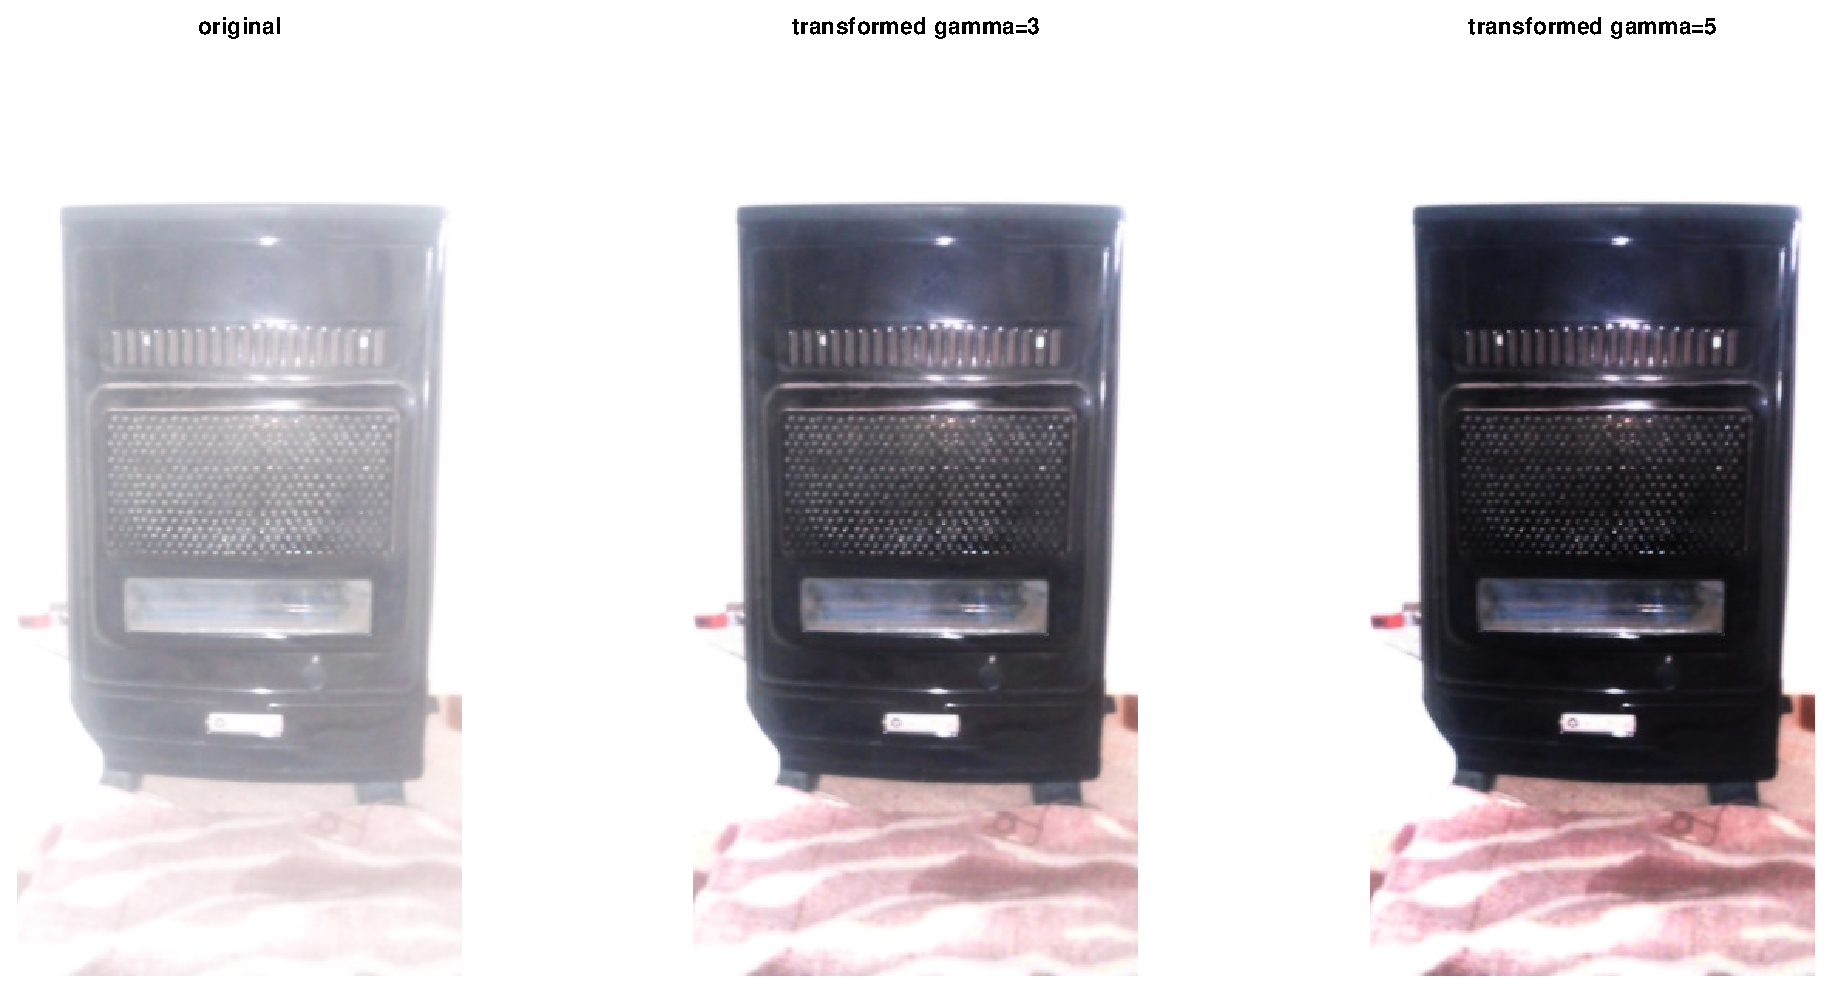
\includegraphics[scale=0.2]{gamma_correction_example.eps}
    \centering
    \caption{gamma correction example}
    \label{fig:gamma_correction_example}
\end{figure}

For processing image, pay attention to the data types. Specially if input is of
type \texttt{int}, the result of pow will be \texttt{int} again and you will 
loss data. So before using pow function, change data to \texttt{double}. Also 
keep the aspect ratio of intensities to avoid exceeding from range of possible 
image data. So it is better to use directly \texttt{im2double} or 
\texttt{mat2gray}.

Inverse function of a gamma transformation is another gamma transformaion. For
example the inverse of $c_1*r^{\gamma_1}$ is $(1/c_1)*r^{1/\gamma_1}$.

If you transform an image by a gamma transformaion and then by its inverse, as
it is predictable, the result will be the original image; because those two
transformations are inverse and their compound is identity function. 
\paragraph*{Note}: Having identity compound needs avoiding data loos during 
transformations.

Gamma transformation with $\gamma < 1$ will increase intensity of darker pixels 
and decrease intensity of lighter pixels. For $\gamma > 1$ it decrease 
intensity of darker pixels and $\dots$ . For $c = \gamma = 1$ transformation is 
identity function.

\subsubsection{Octave notes for gamma transformation}

Suppose we have an image with name \emph{orig} and want to do gamma correction 
like this:

\begin{Verbatim}[frame=single,label=Octave lab:\ bad Gamma correction on Uint image]
    > orig=imread("orig.png");
    > pkg load image;
    > orig=rgb2gray(orig);
    > gamma_corrected_4=orig.^(0.4);
    > figure;subplot(1,2,1);imshow (orig);title ("original")
    > subplot(1,2,2);imshow (gamma_corrected_4);
    title ("corrected:0.4") 
\end{Verbatim}

The result will be like this:

\begin{figure}[htb!]
    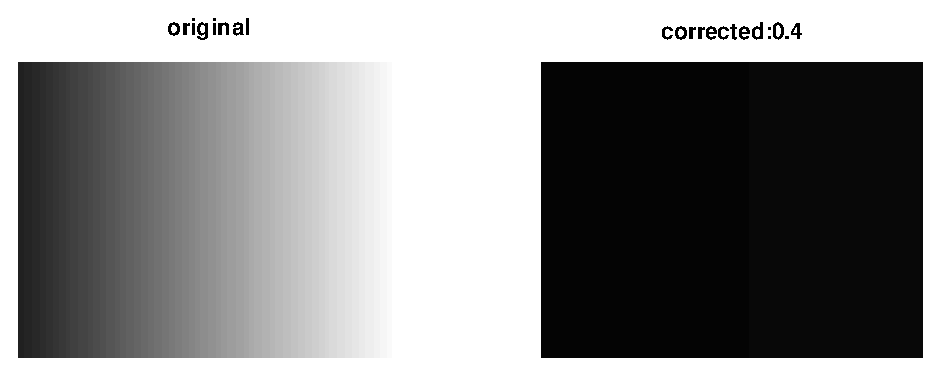
\includegraphics[scale=0.4]{bad_Gamma_correction_on_Uint_image.eps}
    \centering
    \caption{bad Gamma correction on Uint image}
    \label{fig:bad_Gamma_correction_on_Uint_image}
\end{figure}

The strange result is because data type of result of \texttt{pow} function for 
\texttt{int} input will be \texttt{int}:
\begin{Verbatim}
    > class(gamma_corrected_4 )
    ans = uint8
\end{Verbatim}
To solve the problem, we have to change data type of input of pow to 
\texttt{double}:
\begin{Verbatim}
    > gamma_corrected_4=im2double(orig).^(0.4);
    > class(gamma_corrected_4)
    ans = double
    > figure;imshow (gamma_corrected_4);title ("corrected:0.4")
\end{Verbatim}
Result of this code is a white image:
\begin{Verbatim}
    > gamma_corrected=double(orig).^(0.4);
    > figure;imshow (gamma_corrected);
\end{Verbatim}
Result is white; because even output of \texttt{double(orig).\string^(0.4)} 
are of type \texttt{double}; but all greater than $1$.

Another way for doing power law transformation is using \texttt{imadjust} 
function.

The command \texttt{imadjust(A,[],[],3)} is equal to converting image 
\emph{A} to \texttt{double}, then applying \texttt{$\mathsf{r^3}$} (in action 
\texttt{.\string^} operator on image of \texttt{double} data type). In using 
\texttt{imadjust(A,[],[],3)} command, there is no need to convert \emph{A} to 
\texttt{double} no via \texttt{im2double} nor via \texttt{mat2gray} commands.

Notes: 
\begin{itemize}
    \item \texttt{imadjust} keeps data type
    \item All inputs to function \texttt{imadjust}, other than image and 
        $\gamma$, are specified as values between $0$ and $1$, 
        independently of the class of image. If, for example, 
        \emph{f} is of class \texttt{uint8}, then \texttt{imadjust} multiplies 
        its values by $255$ to determine the actual values to use. Using the 
        empty matrix ($[ \ ]$) for $[lowin\ highin]$ or for $[lowOut\ highOut]$ 
        results in the default values $[0 \ 1]$.
    \item \texttt{imadjust} can work on \emph{RGB} image and returns \emph{RGB}

\end{itemize}


